% TEXINPUTS=.:/home/hei2/Documents/LaTeX/myTexStyles:
% created for Journal of Heuristics 
% Time-stamp: "2011-07-18 14:17 hei2"
% if all fonts computer modern use -G1
% dvips -Ppdf -G0 <filename>
% http://www.springer.de/comp/lncs/authors.html

%!TEX TS-program = xelatex
%!TEX encoding = UTF-8 Unicode

%! xelatex joh.tex
%! makeindex joh.nlo -s nomencl.ist -o joh.nls


\RequirePackage{fix-cm} 

\documentclass[smallextended]{llncs}

\usepackage[english]{babel}  
\usepackage{latexsym}
\usepackage{amsmath,amssymb}
\usepackage[dvips]{graphicx,psfrag}
\graphicspath{{figures/}}
\DeclareGraphicsExtensions{.eps}
\usepackage{color}
\usepackage{url}
\include{shorthand} % put your own shorthand declarations in this document


\newcommand{\citet}[1]{\cite{#1}}
\newcommand{\citep}[1]{\cite{#1}}
\newcommand{\citeauthor}[1]{\cite{#1}}

\hyphenpenalty=800
\hbadness=2500


\title{Generating Training Data for Learning Linear Composite Dispatching Rules for Scheduling}
\author{Helga Ingimundardottir \and Thomas Philip Runarsson}

\institute{{School of Engineering and Natural Sciences, University of Iceland}\\
\email{hei2@hi.is} and \email{tpr@hi.is}}

\begin{document}
\maketitle

%\thispagestyle{empty}\pagestyle{empty}
\selectlanguage{english}

\begin{abstract}
A supervised learning approach to generating composite linear priority dispatching rules for scheduling is studied. In particular we investigate a number of strategies for generating training data for learning a linear dispatching rule using preference learning. The results show that generating training data set from optimal solutions only is not as effective as when suboptimal solutions are added to the set. Furthermore, different strategies for creating preference pairs is investigated as well as sub-optimal solution trajectories. The different strategies are investigates on some 2000 randomly generated problem instances using two different problems generator settings.
\end{abstract}

\section{Introduction}
The job-shop scheduling problem (JSP) deals with the allocation of tasks of competing resources where the goal is to 
optimise a single or multiple objectives, in particular minimising a schedule's maximum completion time, i.e. the 
makespan. Due to difficulty in solving this problem heuristics are common applied. Perhaps the simplest approach to 
generating good solutions to the JSP is by applying dispatching rules \cite{Panwalkar77}. For example, dispatching a 
job which has the most work remaining (MWR). Composites of such simple rules can perform significantly better 
\cite{Jayamohan04}. As a consequence a linear composite of dispatching rule was presented by the authors in 
\cite{InRu11a}. There the goal was to learn a set of weights, $\vec{w}$ via logistic regression such that 
\begin{equation}\label{eq:jssp:linweights}
h(\vec{x}_j)=\inner{\vec{w}}{\vphi(\vec{x}_j)},
\end{equation}
yields the preference estimate for dispatching the job $j$ that corresponds to post-decision state $\vec{x}_j$, where 
$\vphi(\vec{x}_j)$ denotes the feature mapping. The features may correspond to a dispatching rule, for example the 
single feature $\phi_1(\vec{x}_j) $ would correspond be the work remaining heuristic if 
$h(\vec{x}_j)>h(\vec{x}_i)$, $\forall i$ are jobs with less work remaining than job $j$. 

The weights in \cite{InRu11a} then found using supervised learning, where the training data was created from optimal 
solutions of randomly generated problem instances. As an alternative would be to minimizing the mean makespan  
directly using a brute force search such as the CMA-ES \citep{Hansen01}. This actually results in a better linear 
composite priority dispatching rules. The nature of the CMA-ES search is to explore suboptimal routes until it 
converges to an optimal one. Implying that the previous approach of only looking into one optimal route may not 
produce a sufficient rich training set. That is, the training set should incorporate a more complete knowledge on 
\emph{all} possible preferences, i.e. make also the distinction between suboptimal and sub-suboptimal features, etc.  
This would require a Pareto ranking of preferences which can be used to make the distinction to which feature sets are 
equivalent, better or worse -- and to what degree, i.e. by giving a weight to the preference. This would results in a 
very large training set, which of course could be re-sampled in order to make it computationally feasible to learn. 
Here we will investigate a number of different ranking strategies for creating preference pairs.

Alternatively, training data could be generated using sub-optimal solution trajectories. For instance~\cite{Siggi05} 
used decision trees to `rediscover' the LPT single priority based dispatching rule by 
using the dispatching rule to create its training data. The limitations of using heuristics to label the training data 
is that the learning algorithm will mimic the original heuristic (both when it works poorly and well on the problem 
instances) and does not consider the real optimum. In order to learn heuristics that can outperform existing 
heuristics, then the training data needs to be correctly labelled. This drawback is confronted 
in~\citep{Malik08,Russell09,Siggi10} by using an optimal scheduler, computed off-line. Here we will both follow 
optimal and sub-optimal solution trajectories, but for each partial solution the preference pair will be labelled 
correctly by solving the partial solution to optimality using a commercial software package \cite{gurobi}.
For this study only MWR, the promising single priority dispatching rule (see~\cite{InRu12a}) for the given data 
distributions, and the CMA-ES found linear dispatching rule will be deemed worthwhile for generating suboptimal 
trajectories.

In summary, the paper considers two main aspects of the generation of the training data, 
\begin{enumerate}
\item how preference pair are created at each decision stage, and
\item which solution trajectorie(s) should be sampled. That is, optimal, random, sub-optimal based on a good 
heuristic, etc.
\end{enumerate}

The paper first illustrated how the JSP problem can be seen as a decision tree where the depth of the tree corresponds 
to the number of job dispatches needed to form a complete schedule. The feature space is also introduced and how 
optimal dispatches and sub-optimal dispatches are labelled as each node in the tree. This is followed by a section 
detailing the strategies investigated in this paper for selecting preference pairs ranking and sampling solution 
trajectories. We then perform an extensive study comparing these strategies, followed by a conclusion and summary of 
main results.



\begin{table}  
  \caption{Feature space $\mathcal{F}$ for JSP where job $J_j$ on machine $M_a$ given the resulting temporal schedule after dispatching $(j,a)$.  }
  \label{tbl:jssp:feat}
  \input{tables/features-description-nomath}
\end{table}

\section{JSP tree representation}\label{sec:gen:gametree}
When building a complete JSP schedule $\ell=n\cdot m$ ($n$ jobs and $m$ machines) dispatches must be made 
sequentially. 
A job is placed at the earliest available time slot for its next machine, whilst still fulfilling constraints that each machine can handle at most one job at each time, and jobs need to have finished their previous machines according to its machine order. 
Unfinished jobs are dispatched one at a time according to some heuristic. After each dispatch\footnote{Dispatch and time step are used interchangeably.} the schedule's current features (cf. Table~\ref{tbl:jssp:feat}) are updated based on the half-finished schedule. 
Fig.~\ref{fig:jssp:gametree} shows how the first two dispatches could be executed for a six-job six-machine job-shop scheduling problem, with the machines, $a\in\{M_1,...,M_6\}$, on the vertical axis and the horizontal axis yields the current makespan. The next possible dispatches are denoted as dashed boxes with the job index $j$ within and its length corresponding to $p_{ja}$.
In the top layer one can see an empty schedule.
In the middle layer one of the possible dispatches from the layer above is fixed, and one can see the resulting 
schedule, i.e. what are the next possible dispatches given this scenario? This sort of tree representation is similar 
to \emph{game trees} \citep{Rosen03} where the root node denotes the initial, i.e. empty, schedule and the leaf nodes 
denote the complete schedule, therefore the distance $k$ from an internal node to the root yields the number of 
operations already dispatched. Traversing from root to leaf node one can obtain a sequence of dispatches that yielded 
the resulting schedule, i.e. the sequence indicates in which order the tasks should be dispatched for that particular 
schedule. 

\begin{figure}[b!]
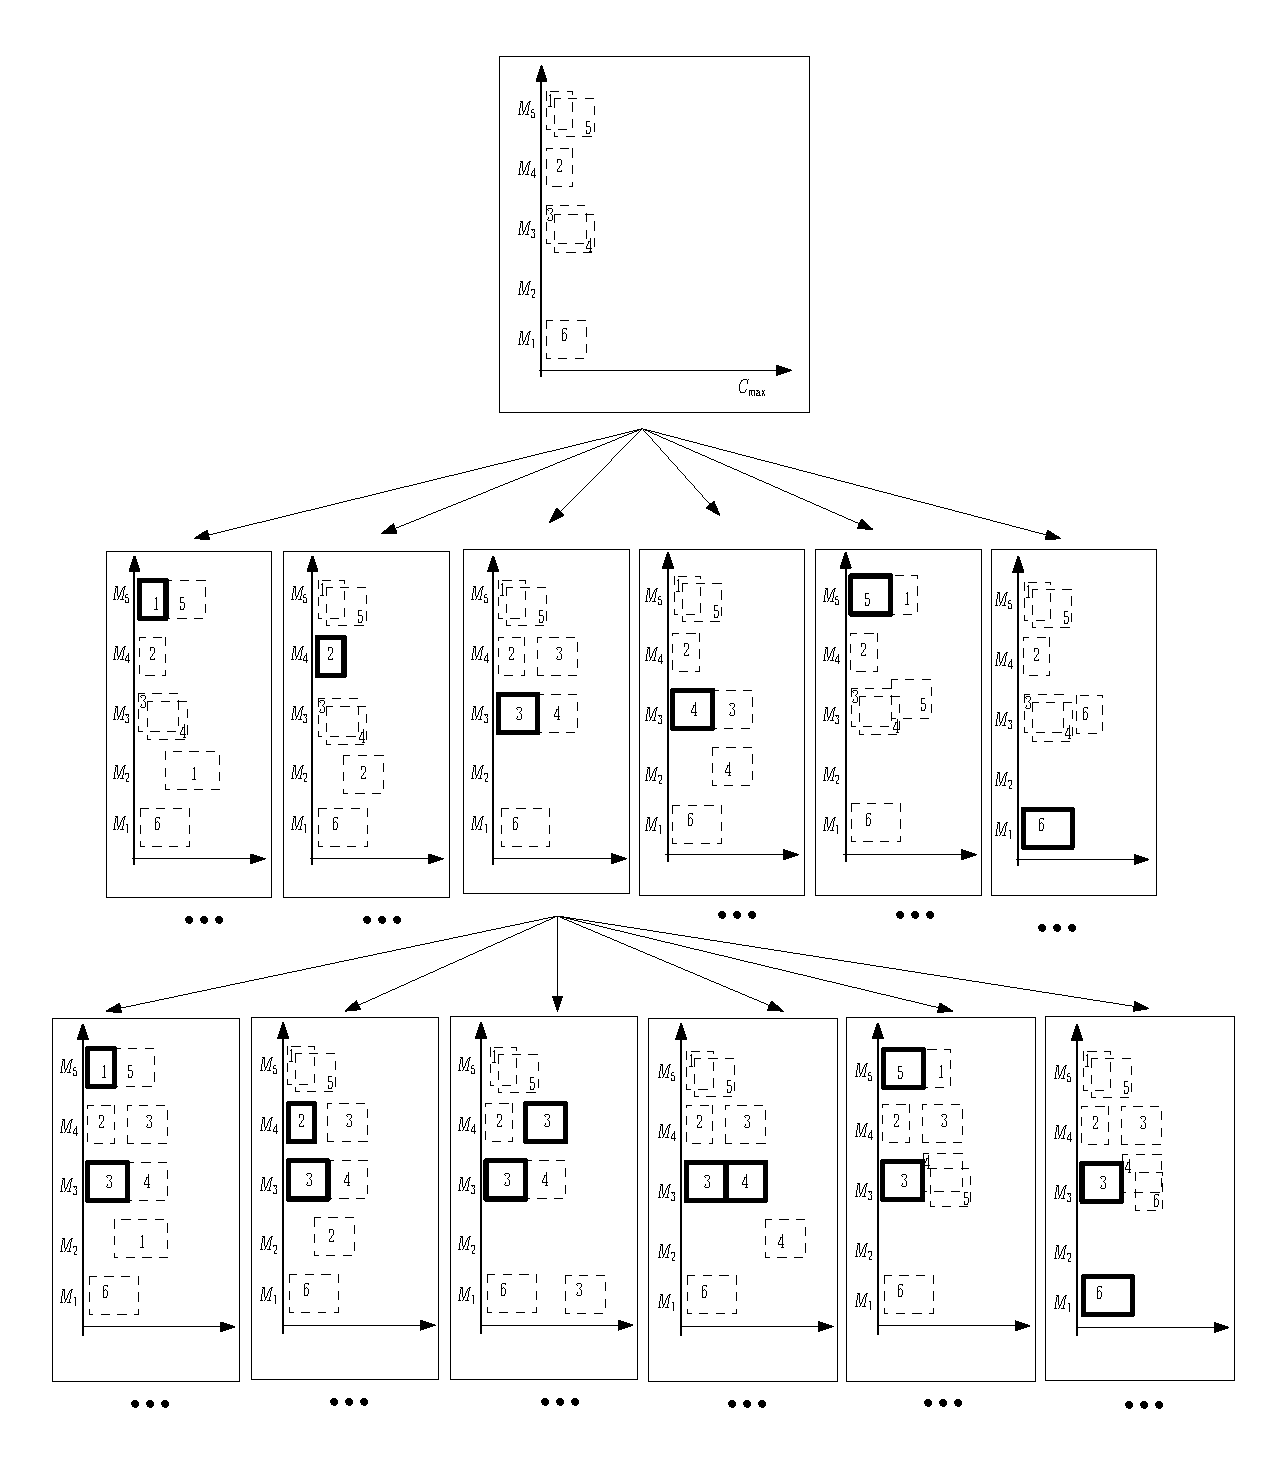
\includegraphics[width=\columnwidth]{gametree}
\caption[Partial Game Tree for JSP]{Partial Tree for job-shop scheduling problem for the first two dispatches. 
Top layer depicts all possible dispatches (dashed) for an empty schedule. 
Middle layer depicts all possible dispatches given that one of the dispatches from the layer above has been executed 
(solid). 
Bottom layer depicts when job $J_3$ on machine $M_4$ has been chosen to be dispatched from the previous layer, 
moreover it depicts all possible next dispatches from that scenario.}
\label{fig:jssp:gametree}
\end{figure}


However, one can easily see that this sequence of task assignments is by no means unique. Inspecting a partial 
schedule further along in the dispatching process such as in Fig.~\ref{fig:jssp:gametree} (top layer), then let's say 
$J_1$ 
would be dispatched next, and in the next iteration $J_2$. Now this sequence would yield the same schedule as if $J_2$ 
would have been dispatched first and then $J_1$ in the next iteration, i.e. these are non-conflicting jobs. Which 
indicates that some of the nodes in the tree can merge. In the meantime the state of the schedules are different and 
thus their features, although they manage to merge with the same (partial) schedule at a later date.  % ATHUGASEMD 1 
%-- SEQ. REP NON-UNIQUE
In this particular instance one can not infer that choosing $J_1$ is better and $J_2$ is worse (or vice versa) since they can both yield the same solution.

Furthermore, in some cases there can be multiple optimal solutions to the same problem instance. Hence not only is the 
sequence representation `flawed' in the sense that slight permutations on the sequence are in fact equivalent w.r.t. 
the end-result, but varying permutations on the dispatching sequence (given the same partial initial sequence) can 
result in very different complete schedules but the same makespan, and thus same deviation from optimality $\rho$ 
defined by~\eqref{eq:ratio}, which is the measure under consideration. Care must be taken in this case that neither 
resulting features are labelled as undesirable or suboptimal. Only the resulting features from a dispatch resulting in 
a suboptimal solution should be labelled undesirable. 

The creation of the tree for job-shop scheduling can be done recursively for all possible permutation of dispatches, 
in the manner described above, resulting in a full \mbox{$n$-ary} tree %(since $|\mathcal{R}|\leq n$)
of height $\ell=n\cdot m$. Such an exhaustive search would yield at the most $n^{\ell}$ leaf nodes (worst case scenario being that no sub-trees merge). Now, since the internal vertices, i.e. partial schedules, are only of interest to learn,\footnote{The root is the empty initial schedule and for the last dispatch there is only one option left to dispatch, so there is no preferred `choice' to learn.} the number of those can be at the most \mbox{${}^{n^{\ell}-1}/_{n-1}$}.
Even for small dimensions of $n$ and $m$ the number of internal vertices are quite substantial and thus 
computationally expensive to investigate them all. 
%Not to mention that this is done iteratively for all $N$ problem instances.



The optimum makespan is known for each problem instance. 
At each time step (i.e. layer of the tree) a number of feature pair are created, they consist of the features 
$\vphi_o$ resulting from optimal dispatches $o\in\mathcal{O}^{(k)}$, versus features $\vphi_s$ resulting from 
suboptimal dispatches $s\in\mathcal{S}^{(k)}$ at time $k$. Note, 
$\mathcal{O}^{(k)}\cup\mathcal{S}^{(k)}=\mathcal{R}^{(k)}$ and $\mathcal{O}^{(k)}\cap\mathcal{S}^{(k)}=\emptyset$.
In particular, each job is compared against another job of the ready-list, $\mathcal{R}^{(k)}$, and if the makespan differs, i.e. $C_{\max}^{(s)}\gneq C_{\max}^{(o)}$, an optimal/suboptimal pair is created, however if the makespan would be unaltered the pair is omitted since they give the same optimal makespan. This way, only features from a dispatch resulting in a suboptimal solution is labelled undesirable.

The approach taken here is to verify analytically, at each time step, by fixing the current temporal schedule as an initial state, whether it can indeed \emph{somehow} yield an optimal schedule by manipulating the remainder of the sequence. This also takes care of the scenario that having dispatched a job resulting in a different temporal makespan would have resulted in the same final makespan if another optimal dispatching sequence would have been chosen. That is to say the data generation takes into consideration when there are multiple optimal solutions to the same problem instance. 

\section{Selecting preference pairs}\label{sec:S:strategies}
At each dispatch iteration $k$ a number of preference pairs are created which can then be multiplied by the number of problem instance $N$ created. A separate data set is deliberately created for each dispatch iterations, as the initial feeling is that dispatch rules used in the beginning of the schedule building process may not necessarily be the same as in the middle or end of the schedule. As a result there are $\ell$ linear scheduling rules for solving a $n \times m$ job-shop.
Defining the size of the preference set as $l=\abs{S}$ (cf.~\cite{InRu11a}). If $l$ is too large, then re-sampling may 
need to be done in order for the ordinal regression to be computationally feasible. 


% % % Iðm assuming that this was not done.!
%Due to the nature of the sequence representation, the earlier stages of the dispatching are more or less equivalent 
%(and thus irrelevant), hence it is appropriate to follow some random optimal path to begin with and then follow some 
%(if not all possible) optimal paths until completion at step $\ell$. The strategy approached in  \cite{InRu11a} was 
%to 
%follow some optimal job $J_j\in\mathcal{O}^{(k)}$, thus creating 
%$\abs{\mathcal{O}^{(k)}}\cdot\abs{\mathcal{S}^{(k)}}$ 
%feature pairs at each dispatch $k$. %, resulting in a training size of,
%\begin{equation}\label{eq:sizeS_b}
%l =  \sum_{i=1}^N \left(2 \abs{\mathcal{O}^{(k)}_i}\cdot \abs{\mathcal{S}^{(k)}_i} \right)
%\end{equation}


\subsection{Ranking strategies}
The following ranking strategies were implemented for adding preference pairs to $S$,
\begin{description}
\item[$S_b$] all optimum rankings $r_1$ versus all possible sub-optimum rankings $r_i$, $i\in\{2,\ldots,n'\}$, preference pairs are added, i.e. same basic set-up as in~\cite{InRu11a}. %Note, $|S_b|$ is defined in~\eqref{eq:sizeS_b}.
\item[$S_f$] full subsequent rankings, i.e. all possible combinations of $r_i$ and $r_{i+1}$ for $i\in\{1,\ldots,n'\}$, preference pairs are added.
\item[$S_p$] partial subsequent rankings, i.e. sufficient set of combinations of $r_i$ and $r_{i+1}$ for $i\in\{1,\ldots,n'\}$, are added to the training set -- e.g. in the cases that there are more than one operation with the same ranking, only one of that rank is needed to compared to the subsequent rank. Note that $S_p\subset S_f$.
\end{description}
where $r_1>r_2>\ldots>r_{n'}$ ($n'\leq n$) are the rankings of the ready-list, $\mathcal{R}^{(k)}$, at time step $k$.

\subsection{Trajectory sampling strategies}
The following trajectory sampling strategies were explored for adding preference pairs to $S$,
\begin{description}
\item[$S^{opt}$] at each dispatch some (random) optimal task is dispatched.
\item[$S^{cma}$] at each dispatch the task corresponding to highest priority, computed with fixed weights $\vec{w}$, which were obtained by optimising the mean for~\eqref{eq:ratio} with CMA-ES. 
\item[$S^{mwr}$] at each dispatch the task corresponding to most work remaining is dispatched, i.e. following the simple dispatching rule MWR.
\item[$S^{rnd}$] at each dispatch some random task is dispatched.
\end{description}
In the case of $S^{mwr}$ and $S^{cma}$ it is sufficient to explore each trajectory exactly once for each problem instance. Whereas, for $S^{opt}$ and $S^{rnd}$ there can be several trajectories worth exploring, however, only one is chosen (at random). It is noted that since the number of problem instances $N$ is large, it is deemed sufficient to explore one trajectory for each instance, in those cases as well.

\section{Experimental study}\label{sec:expr:locallin}

For $N$ problem instances generated using $n$ jobs and $m$ machines for processing times 
following the same distribution and random $\sigma$ permutations of job orderings. The optimum makespan is denoted 
$C_{\max}^{\text{opt}}$, and the makespan obtained from the linear learning model by $C_{\max}^{\text{model}}$. Since 
the optimal makespan varies between problem instances the performance measure is the following, 
\begin{equation}\label{eq:ratio}\rho=\frac{C_{\max}^{\text{model}}-C_{\max}^{opt}}{C_{\max}^{\text{opt}}}\cdot 
100\%\end{equation}
which indicates the percentage relative deviation from optimality. 


To test the validity of different ranking and strategies from section~\ref{sec:S:strategies}, a training set of 
$N_{\text{train}}=500$ and $N_{\text{test}}=500$ problem instances of $6\times 5$ job-shop for several problem space 
distributions, namely $\mathcal{P}_1$ and $\mathcal{P}_2$, where processing are drawn from a uniform distribution 
$\mathcal{U}(10,100)$ and $\mathcal{U}(50,100)$ respectively. 
The size of the preference set, $S$, for different trajectory and ranking strategies is depicted in Fig.~\ref{fig:sizeofprefset:p1} and ~\ref{fig:sizeofprefset:p2}, for $\mathcal{P}_1$ and $\mathcal{P}_2$, respectively. 

A linear ordinal regression model was created for each preference set, $S$, for problem space $\mathcal{P}_1$. A box-plot with the results of percentage relative deviation from optimality, $\rho$, defined by~\eqref{eq:ratio}, is presented in Fig.~\ref{fig:track:boxplot:p1} and~\ref{fig:rank:boxplot:p1}. Fig.~\ref{fig:track:boxplot:p1} depicts different ranking strategies for a fixed trajectory, whereas Fig.~\ref{fig:rank:boxplot:p1} depicts different trajectory strategies for a fixed ranking. 
From the figures it is apparent there can be a performance edge gained by implementing a particular ranking or trajectory strategy, moreover the behaviour is analogous across different disciplines. Similarly, Fig.~\ref{fig:track:boxplot:p2} and~\ref{fig:rank:boxplot:p2} for problem space $\mathcal{P}_2$.

Note that $S_{all}$ denotes that all rankings were explored, i.e. $S_{all}=S_b\cup S_f\cup S_p$. Similarly, $S^{all}=S^{opt}\cup S^{cma}\cup S^{mwr} \cup S^{rnd}$ for all trajectories.

\begin{figure} \centering
\includegraphics[width=0.49\textwidth]{sizeS_opt_p1}
\includegraphics[width=0.49\textwidth]{sizeS_CMA_p1} \\
\hfill $S^{opt}$ \hfill $S^{cma}$  \\
\includegraphics[width=0.49\textwidth]{sizeS_MWR_p1}
\includegraphics[width=0.49\textwidth]{sizeS_rnd_p1}\\
\hfill $S^{mwr}$ \hfill $S^{rnd}$
\caption{Size of preference set, $l$ for different trajectory and ranking strategies ($S_b$ in blue, $S_f$ in red, $S_p$ in green), given problem space $\mathcal{P}_1$, where $N_{\text{train}}=500$.}
\label{fig:sizeofprefset:p1}
\end{figure}

\begin{figure} \centering
\includegraphics[width=0.49\textwidth]{sizeS_opt_p2}
\includegraphics[width=0.49\textwidth]{sizeS_CMA_p2} \\
\hfill $S^{opt}$ \hfill $S^{cma}$  \\
\includegraphics[width=0.49\textwidth]{sizeS_MWR_p2}
\includegraphics[width=0.49\textwidth]{sizeS_rnd_p2}\\
\hfill $S^{mwr}$ \hfill $S^{rnd}$
\caption{Size of preference set, $l$ for different trajectory and ranking strategies ($S_b$ in blue, $S_f$ in red, $S_p$ in green), given problem space $\mathcal{P}_2$, where $N_{\text{train}}=500$.}
\label{fig:sizeofprefset:p2}
\end{figure}

% % p1
\begin{figure}\flushright \hfill
\includegraphics[width=0.49\textwidth]{histTrack_train_p1} \hfill
\includegraphics[width=0.49\textwidth]{histTrack_test_p1} \\
\hfill {Training set }\hfill {Testing set}
\caption{Box-plot of results for linear ordinal regression model trained on various preference sets using problem space $\mathcal{P}_1$. Note that same trajectory schemes are colour-coded the same.}
\label{fig:track:boxplot:p1}
\end{figure}

\begin{figure}\flushright \hfill
\includegraphics[width=0.49\textwidth]{histRank_train_p1} \hfill
\includegraphics[width=0.49\textwidth]{histRank_test_p1} \\
\hfill {Training set }\hfill {Testing set}
\caption{Box-plot of results for linear ordinal regression model trained on various preference sets using problem space $\mathcal{P}_1$. Note that same ranking schemes are colour-coded the same.}
\label{fig:rank:boxplot:p1}
\end{figure}
% % p2
\begin{figure}\flushright \hfill
\includegraphics[width=.45\textwidth]{histTrack_train_p2} \hfill
\includegraphics[width=.45\textwidth]{histTrack_test_p2} \\
\hfill {Training set } \hfill {Test set }
\caption{Box-plot of results for linear ordinal regression model trained on various preference sets using problem space $\mathcal{P}_2$. }
\label{fig:track:boxplot:p2}
\end{figure}
 
\begin{figure}\flushright \hfill
\includegraphics[width=0.49\textwidth]{histRank_train_p2} \hfill
\includegraphics[width=0.49\textwidth]{histRank_test_p2} \\
\hfill {Training set }\hfill {Testing set}
\caption{Box-plot of results for linear ordinal regression model trained on various preference sets using problem space $\mathcal{P}_2$. }
\label{fig:rank:boxplot:p2}
\end{figure}

\subsection{Ranking strategies}
There is no statistical difference between $S_f$ and $S_p$ ranking-schemes across all disciplines (cf. 
Fig.~\ref{fig:track:boxplot:p1} and~\ref{fig:track:boxplot:p2}), which is expected since $S_f$ is designed to contain 
the same preference information as $S_f$. However neither of the Pareto ranking-schemes outperform the original $S_b$ 
set-up from~\cite{InRu11a}. The results hold for both test and training sets. 

Combining the ranking schemes, $S_{all}$, improves the individual ranking-schemes across all disciplines, except in the case of $S_b^{opt}\big|_{\mathcal{P}_1}$ and $S_b^{rnd}\big|_{\mathcal{P}_2}$, in which case there were no statistical difference. Now, for the test set, the results hold, however there is no statistical difference between $S_b$ and $S_{all}$ for most trajectories $\{S^{opt},S^{cma},S^{rnd}\}\big|_{\mathcal{P}_1}$ and  $\{S^{opt},S^{rnd}\}\big|_{\mathcal{P}_2}$. Now, whereas a smaller preference set is preferred, its opted to use the $S^{b}$ ranking scheme. 

Moreover, it is noted that the learning algorithm is able to significantly outperform the original heuristics, MWR and CMA-ES (white), used to create the training data $S^{mwr}$ (grey) and $S^{cma}$ (yellow), respectively (cf. Fig.~\ref{fig:track:boxplot:p1} and~\ref{fig:track:boxplot:p2}). For both $\mathcal{P}_1$ and $\mathcal{P}_2$, linear ordinal regression models based on $S^{mwr}$ are significantly better than $MWR$, irrespective of the ranking schemes. Whereas the fixed weights found via CMA-ES are only outperformed by linear ordinal regression models based on $\{S_b^{cma},S_{all}^{cma}\}$. This implies that ranking scheme needs to be selected appropriately. Result hold for the test data.

\subsection{Trajectory sampling strategies}
Learning preference pairs from a good scheduling policies, such as $S^{cma}$ and $S^{mwr}$, gave considerably more favourable results than tracking optimal paths (cf. Fig.~\ref{fig:track:boxplot:p1} and~\ref{fig:track:boxplot:p1}). Suboptimal routes are preferred when dealing with $\mathcal{P}_1$ (for all ranking schemes), however when encountering $\mathcal{P}_2$ the choice of ranking schemes can yield the exact opposite.

It is particularly interesting there is no statistical difference between $S^{opt}$ and $S^{rnd}$ for both 
$\{S_{b},S_{f}\}\big|_{\mathcal{P}_1}$ and $\{S_b,S_f,S_p\}\big|_{\mathcal{P}_2}$ ranking-schemes. That is to say, 
tracking optimal dispatches gives the same performance as completely random dispatches. This indicates that exploring 
only optimal trajectories can result in a training set where the learning algorithm is inept to determine good 
dispatches in the circumstances when newly encountered features have diverged from the learned feature set labelled to 
optimum solutions. 

Finally, $S^{all}$ gave the best combination across all disciplines. Adding suboptimal trajectories with the optimal trajectories gives the learning algorithm a greater variety of preference pairs for getting out of local minima.

\subsection{Following CMA-ES guided trajectory}
The rational for using the $S^{cma}$ strategy was mostly due to the fact a linear classifier is creating the training data (using the weights found via CMA-ES optimisation), hence the training data created should be linearly separable, which in turn should boost the training accuracy for a linear classification learning model. However, this strategy is easily outperformed by the single priority based dispatching rule MWR guiding the training data collection, $S^{mwr}$. 

Let's inspect the CMA-ES guided training data more closely, in particular the linear weights for~\eqref{eq:jssp:linweights}. The weights are depicted in Fig.~\ref{fig:weights:p1} and~\ref{fig:weights:p2} for problem space $\mathcal{P}_1$ and $\mathcal{P}_2$, respectively. The original weights found via CMA-ES optimisation, that are used to guide the collection of training data, are depicted in red and  weights obtained by the linear classification model for $S_b^{cma}$ are depicted in blue.

From the CMA experiments it is clear that a lot of weight is applied to the $w_6$ that corresponds implementing MWR, yet the existing weights for other features diverges the training data from a more ``better'' training set to learn. Arguably, it might be due to the computational cost involved in implementing CMA-ES, meaning that even after 1,500 function evaluations the method might still be far from optimum weights. It might also be an artefact due the fact the training set during the CMA-ES search is different to the data generation described in Sec.~\ref{sec:S:strategies} is completely different, hence the different scaling parameters for the features might influence the results. Moreover, the CMA-ES is minimizing the makespan directly, whereas the supervised linear models are learning to discriminate optimal versus suboptimal features sets that implies a better deviation from optimality later on. 

\begin{figure}\centering
\includegraphics[width=0.12\textwidth]{weights/p1w1}
 \includegraphics[width=0.12\textwidth]{weights/p1w2}
 \includegraphics[width=0.12\textwidth]{weights/p1w3}
 \includegraphics[width=0.12\textwidth]{weights/p1w4}
 \includegraphics[width=0.12\textwidth]{weights/p1w5}
 \includegraphics[width=0.12\textwidth]{weights/p1w6}
 \includegraphics[width=0.12\textwidth]{weights/p1w7}
 \includegraphics[width=0.12\textwidth]{weights/p1w8}
 \includegraphics[width=0.12\textwidth]{weights/p1w9}
 \includegraphics[width=0.12\textwidth]{weights/p1w10}
 \includegraphics[width=0.12\textwidth]{weights/p1w11}
 \includegraphics[width=0.12\textwidth]{weights/p1w12}
 \includegraphics[width=0.12\textwidth]{weights/p1w13}
\caption{Linear weights for $\mathcal{P}_1$. Weights ($w_1$ to $w_{13}$ from left to right, top to bottom) found via CMA-ES optimisation (red), and weights found via learning classification model based on $S_b^{cma}$ (blue). }\label{fig:weights:p1}
\end{figure}

\begin{figure}\centering
\includegraphics[width=0.12\textwidth]{weights/p2w1}
 \includegraphics[width=0.12\textwidth]{weights/p2w2}
 \includegraphics[width=0.12\textwidth]{weights/p2w3}
 \includegraphics[width=0.12\textwidth]{weights/p2w4}
 \includegraphics[width=0.12\textwidth]{weights/p2w5}
 \includegraphics[width=0.12\textwidth]{weights/p2w6}
 \includegraphics[width=0.12\textwidth]{weights/p2w7}
 \includegraphics[width=0.12\textwidth]{weights/p2w8}
 \includegraphics[width=0.12\textwidth]{weights/p2w9}
 \includegraphics[width=0.12\textwidth]{weights/p2w10}
 \includegraphics[width=0.12\textwidth]{weights/p2w11}
 \includegraphics[width=0.12\textwidth]{weights/p2w12}
 \includegraphics[width=0.12\textwidth]{weights/p2w13}
\caption{Linear weights for $\mathcal{P}_2$. Weights  ($w_1$ to $w_{13}$ from left to right, top to bottom) found via CMA-ES optimisation in red, and weights found via learning classification model based on $S_b^{cma}$ in blue.}\label{fig:weights:p2}
\end{figure}

\subsection{Summary and conclusion}
As the experimental results illustrate in section~\ref{sec:expr:locallin}, the ranking of optimal\footnote{Here the 
tasks labelled `optimal' do not necessarily yield the optimum makespan (except in the case of following optimal 
trajectories), instead these are the optimal dispatches for the given partial schedule.} and suboptimal features are 
of paramount importance. The subsequent rankings are not of much value, since they are disregarded anyway. However, 
the trajectories to create training instances have to be varied.

Unlike~\citep{Siggi10,Malik08,Russell09}, learning only on optimal training data was not fruitful. However, inspired 
by the original work by~\cite{Siggi05}, having heuristic guide the generation of training data, but with nevertheless 
optimal labelling based on a solver, gave meaningful preference pairs which the learning algorithm could learn. In 
conclusion, henceforth, the training data will be generate with $S_{b}^{all}$ scheme for the authors' future work.

Based on these preliminary experiments, we continue to test on a greater variety of problem data distributions for 
scheduling, namely job-shop and permutation flow-shop problems. Once training data has been carefully created, global 
dispatching rules can finally be learned, with the hope of implementing them for a greater number of jobs and 
machines. This is the focus of our current work.

\footnotetext{A note to the reviewer of this paper: we know that some of the figures have too small fonts and are in 
colour, this will be fixed in the final version (we still have room for 2.5 more pages).}

\bibliographystyle{splncs} 
\begin{thebibliography}{10}

\bibitem{Panwalkar77}
Panwalkar, S.S., Iskander, W.:
\newblock A survey of scheduling rules.
\newblock Operations Research \textbf{25}(1) (1977)  45--61

\bibitem{Jayamohan04}
Jayamohan, M., Rajendran, C.:
\newblock Development and analysis of cost-based dispatching rules for job shop
  scheduling.
\newblock European Journal of Operational Research \textbf{157}(2) (2004)
  307--321

\bibitem{InRu11a}
Ingimundardottir, H., Runarsson, T.P.:
\newblock Supervised learning linear priority dispatch rules for job-shop
  scheduling.
\newblock In Coello, C., ed.: Learning and Intelligent Optimization. Volume
  6683 of Lecture Notes in Computer Science.
\newblock Springer Berlin, Heidelberg (2011)  263--277

\bibitem{Hansen01}
Hansen, N., Ostermeier, A.:
\newblock Completely derandomized self-adaptation in evolution strategies.
\newblock Evol. Comput. \textbf{9}(2) (June 2001)  159--195

\bibitem{Siggi05}
Li, X., Olafsson, S.:
\newblock Discovering dispatching rules using data mining.
\newblock Journal of Scheduling \textbf{8} (2005)  515--527

\bibitem{Malik08}
Malik, A.M., Russell, T., Chase, M., Beek, P.:
\newblock Learning heuristics for basic block instruction scheduling.
\newblock Journal of Heuristics \textbf{14}(6) (December 2008)  549--569

\bibitem{Russell09}
Russell, T., Malik, A.M., Chase, M., van Beek, P.:
\newblock Learning heuristics for the superblock instruction scheduling
  problem.
\newblock IEEE Trans. on Knowl. and Data Eng. \textbf{21}(10) (October 2009)
  1489--1502

\bibitem{Siggi10}
Olafsson, S., Li, X.:
\newblock Learning effective new single machine dispatching rules from optimal
  scheduling data.
\newblock International Journal of Production Economics \textbf{128}(1) (2010)
  118--126

\bibitem{gurobi}
{Gurobi Optimization, Inc.}:
\newblock Gurobi optimization (version 5.0) [software] (May 2012)

\bibitem{InRu12a}
Ingimundardottir, H., Runarsson, T.P.:
\newblock {Determining the Characteristic of Difficult Job Shop Scheduling
  Instances for a Heuristic Solution Method}.
\newblock In Schoenauer, M., ed.: Learning and Intelligent Optimization, 6th
  International Conference, LION 6, Paris, Springer Lecture Notes in Computer
  Science (2012)

\bibitem{Rosen03}
Rosen, K.H.:
\newblock 9.
\newblock In: Discrete Mathematics and Its Applications. 5 edn. McGraw-Hill,
  Inc., New York, NY, USA (2003)  631--700

\end{thebibliography}



\end{document}

